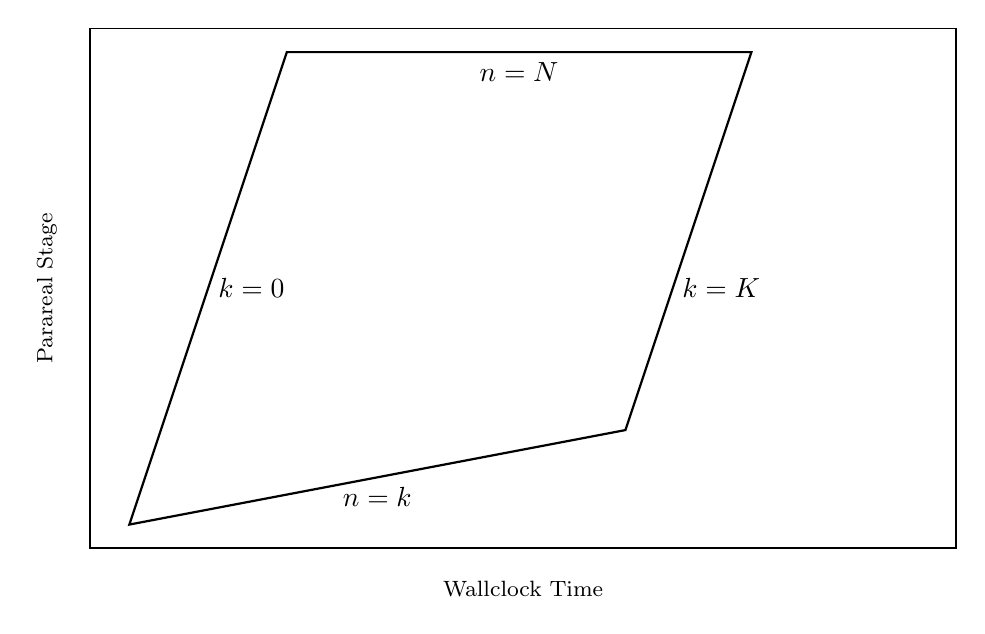
\begin{tikzpicture}
  %\def\mxscale{0.6}
  \def\myscale{0.6}
%\begin{scope}[xscale=\mxscale]
  % axis and labels
  \node[below] at (5,-0.5*\myscale-0.3) {\footnotesize Wallclock Time};
  \node[rotate=90, above] at (-0.5-0.3,5*\myscale) {\footnotesize Parareal Stage};
\begin{scope}[yscale=\myscale]
  \draw[semithick] (-0.5,-0.5) rectangle (10.5,10.5);
  % timeline diagram
  \draw[thick] (0,0)
    -- node[right] {$k=0$} (2,10)
    -- node[below] {$n=N$} (7.9,10)
    -- (6.3,2)
    -- node[below] {$n=k$} cycle;
  \node[right] at (6.9,5) {$k=K$};
  %\draw[gray,thick,dashed] (6.3,2) -- (9.45,3);
  %\draw[gray,thick,dashed] (7.9,10) -- (9.45,10);
\end{scope}
%\end{scope}
\end{tikzpicture}
